\section{Experimentación Y Resultados}

A continuación expondremos los resultados obtenidos por cada algoritmo para distintas imágenes. El objetivo será posteriormente hacer análisis de calidad subjetiva (es decir que vemos a simple vista), objetiva y tiempo de computos. Para, como dijimos en un principio, determinar ventajas y desventajas de cada uno de ellos. Para los análisis objetivos desarrollamos un programa en python que compara pixel a pixel basado en PSNR (Peak signal-to-noise ratio). 

\subsection{PNSR}
Es un método para definir la relación entre una señal y el ruido de la regenaración de la misma expresado en decibeles. En este caso, así como es comunmente utilizado, sirve para resolver si la imagen final es "parecida" a la original. Es importante notar que a medida que mayor sea el resultado, mejor es la calidad de la imágen.

\subsection{Colores}


Se nos ocurrió que podría ser interesante chequear los comportamientos de estos procedimientos en una imagen con muchos bordes ya que estos, en algoritmos como el directional, son factores importantes y potencialmente conflictivos. Además hicimos que la imagen sea grande (5000 x 3000 pixeles) para poder analizar tiempos de computo y para influir en la calidad subjetiva, ya que si ponemos imágenes con mucha definición pequeños errores podrían pasar desapercividos para el ojo humano.

Tambien expondremos la imagen bayerizada para que quede claro que la conversción que estamos haciendo es correcta.

\begin{figure}

\minipage{0.5\textwidth}
\begin{center}
       
\includegraphics[scale=0.04]{imagenes/colores.png}
       \caption{Original }\label{fig:awesome_image1}
        \end{center}
\endminipage\hfill
\minipage{0.5\textwidth}
\begin{center}
        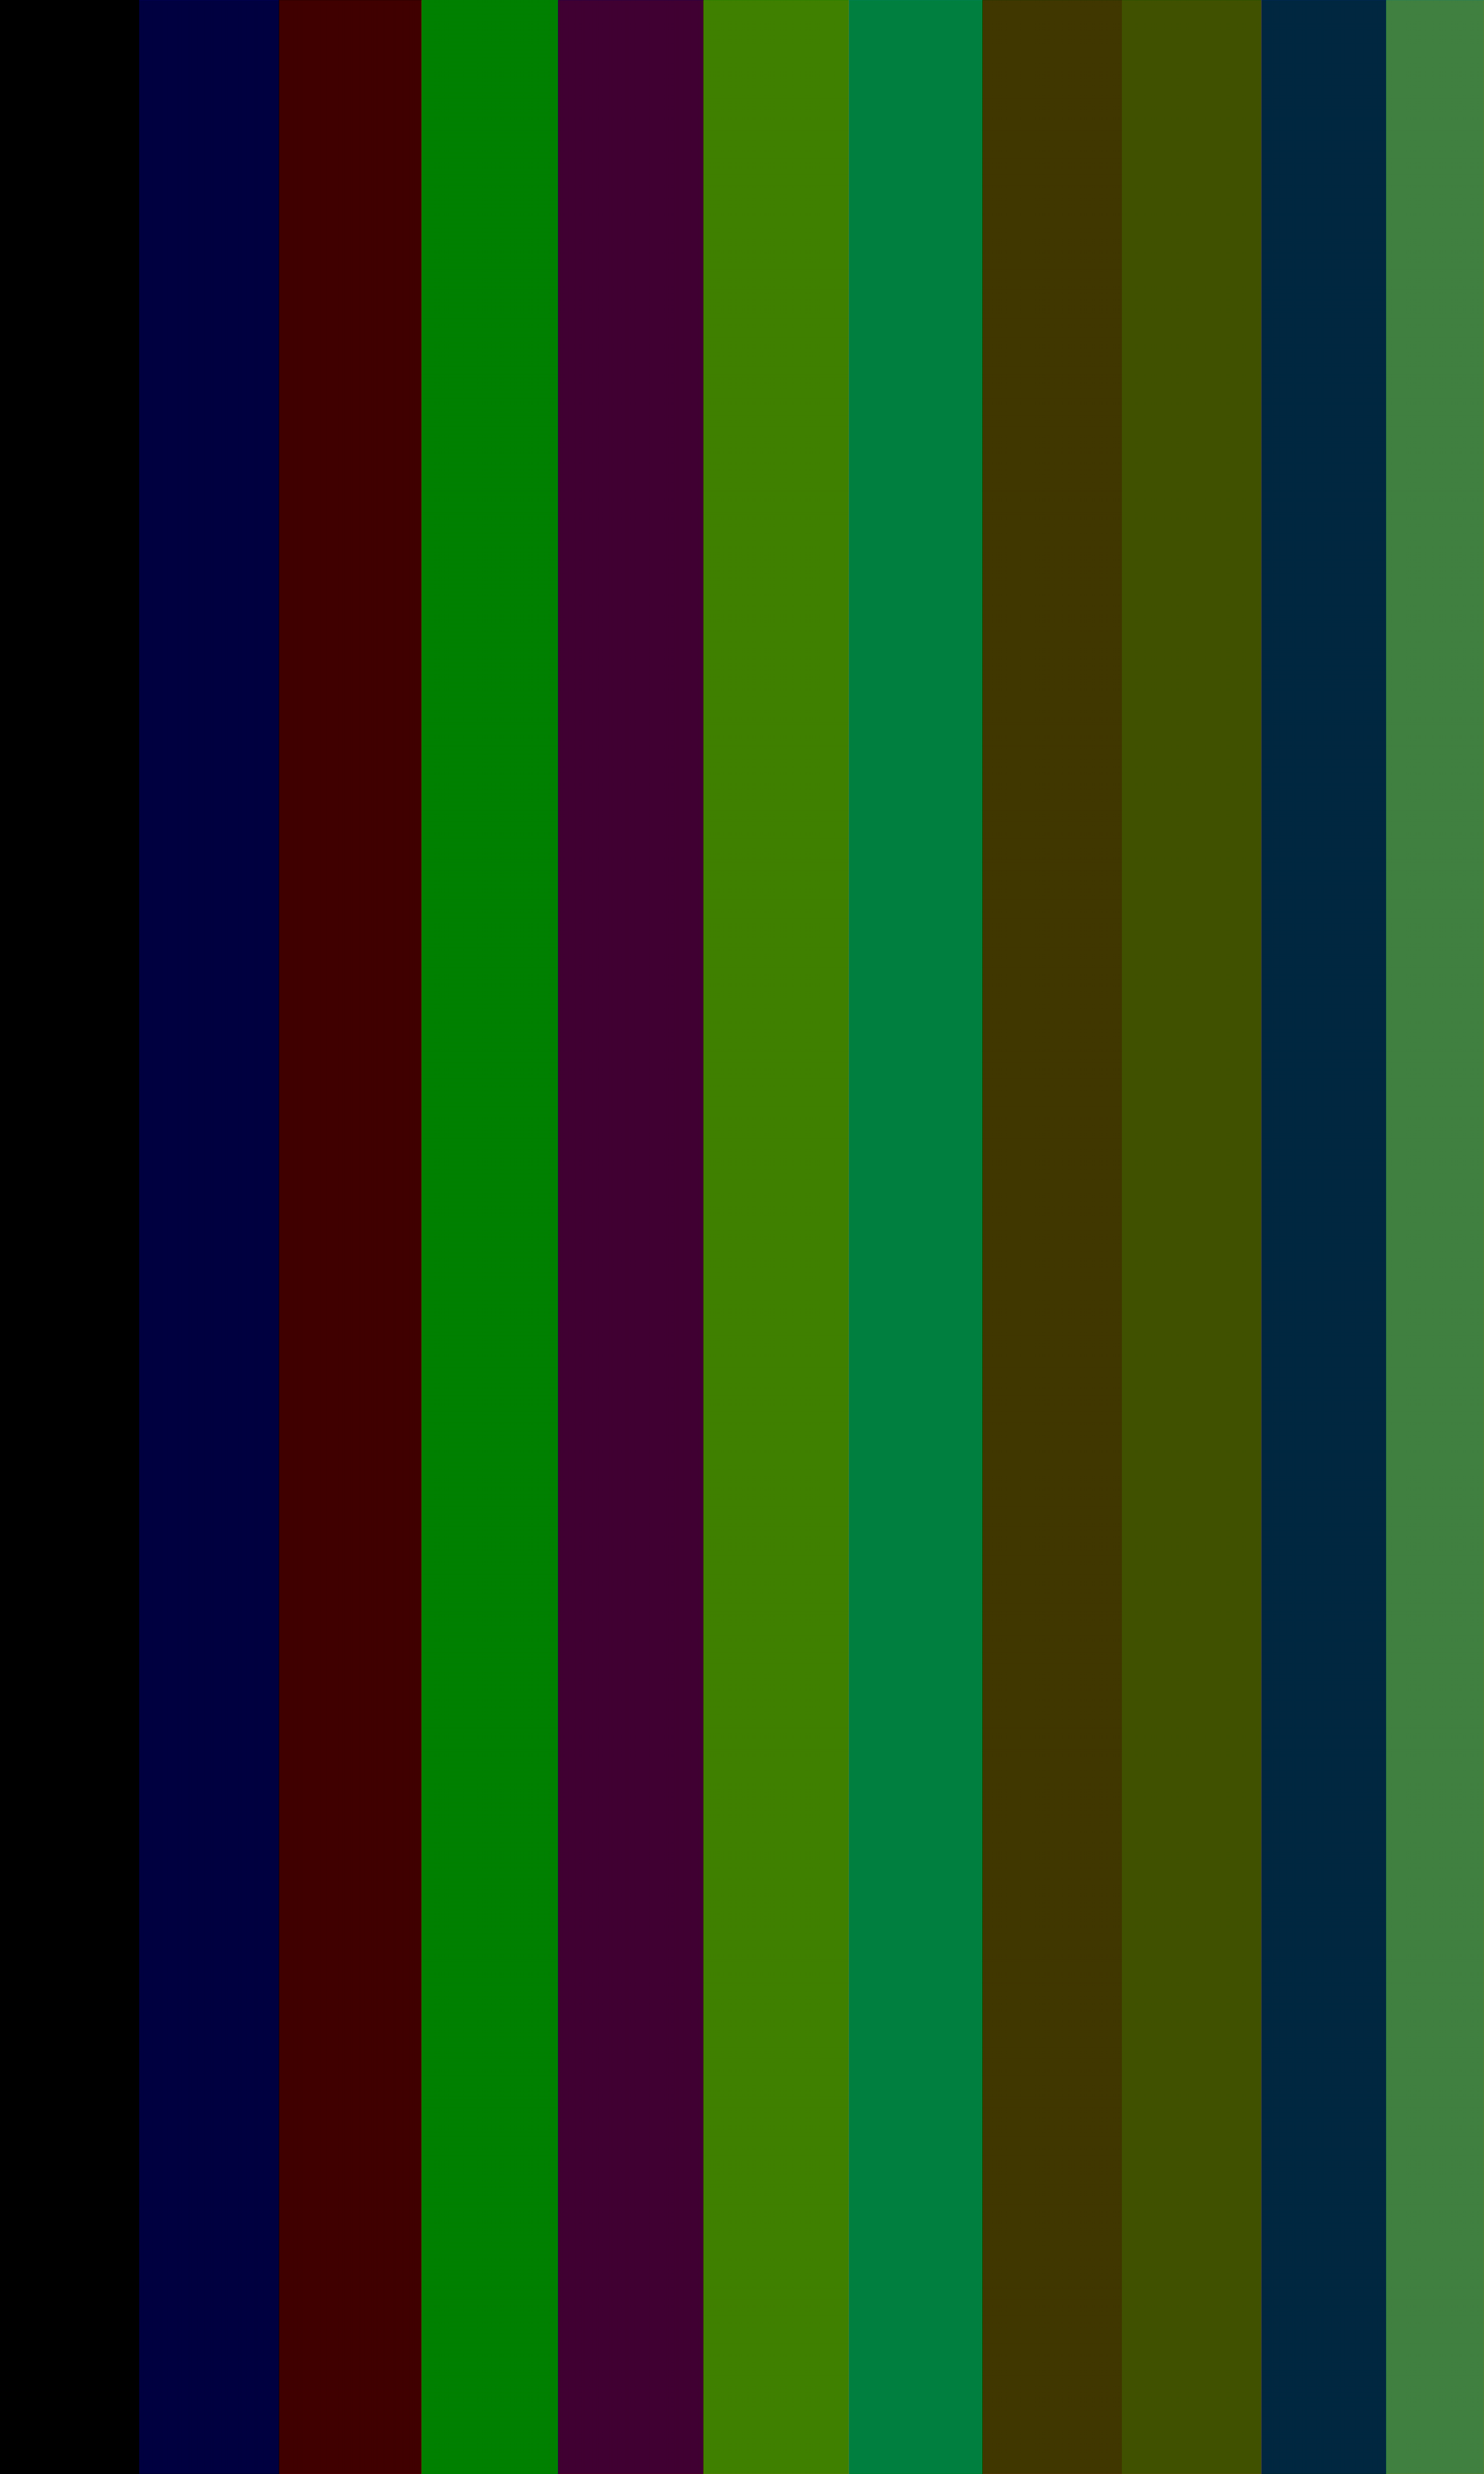
\includegraphics[scale=0.04]{imagenes/colores_bayer.png}
       \caption{Bayerizada}\label{fig:awesome_image1}
        \end{center}
\endminipage\hfill 
\end{figure}
\newpage
\begin{figure}[!htb]
\minipage{0.5\textwidth}
\begin{center}
    
\includegraphics[scale=0.04]{imagenes/colores_demosicing_bilineal.png}
    \caption{Bilineal }
 \end{center}
\endminipage
\minipage{0.5\textwidth}
\begin{center}
    
\includegraphics[scale=0.04]{imagenes/colores_demosicing_quality.png}
    \caption{High Quality}
        \end{center}
\endminipage\hfill
\end{figure}

\begin{figure}
\minipage{0.5\textwidth}
\begin{center}
    
\includegraphics[scale=0.04]{imagenes/colores_demosicing_spline.png}
    \caption{Directional}
        \end{center}
\endminipage
\minipage{0.5\textwidth}
\begin{center}
    
\includegraphics[scale=0.04]{imagenes/colores_demosicing_vecino.png}
    \caption{Vecinos}
 \end{center}
\endminipage
 
\end{figure}
\newpage

Efectivamente a primera vista parecería que todas dieran lo mismo. Pero veamos que si le hacemos zoom, no es así.
\begin{figure}[!htb]
\minipage{0.5\textwidth}
\begin{center}
    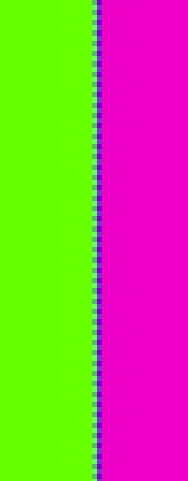
\includegraphics[scale=0.6]{imagenes/colores_bilineal_zoom.jpg}
    \caption{Bilineal Zoom}
        \end{center}
\endminipage
\minipage{0.5\textwidth}
\begin{center}
    
\includegraphics[scale=0.6]{imagenes/colores_hq_zoom.jpg}
    \caption{Bilineal Zoom}
        \end{center}
\endminipage 
\end{figure}
\newpage
\begin{figure}[!htb]
\minipage{0.5\textwidth}
\begin{center}
    
\includegraphics[scale=0.6]{imagenes/colores_directional_zoom.jpg}
    \caption{Directional Zoom}
        \end{center}
\endminipage
\minipage{0.5\textwidth}
\begin{center}
    
\includegraphics[scale=0.6]{imagenes/colores_vecinos_zoom.jpg}
    \caption{Vecinos Zoom}
        \end{center}
\endminipage 
\end{figure}


El algoritmo bilineal y el high quality tuvieron pequeños errores en los bordes. Podemos observar que en esos casos entre el verde y el violeta parece haber como una `cosedura', la misma se repite en todos los bordes de la imagen. Estas diferencias imperceptibles por el tamaño de la imagen a primera vista pueden ser efectivamente comprobadas mediante un análisis de calidad objetivo. 

A continuación podemos ver los PSNR obtenidos al comparar los distintos resultados con la imagen original. Las im{ágenes que al hacerles zoom tenían esas "coseduras" efectivamente fueron las que mas bajo PSNR dieron, es decir las que mas difirieron de la real.

$$ 
\begin{bmatrix}
           &      PSNR     \\
       quality    &   39.67   \\
       bilineal    &      41.14   \\
       directional    &      48.13    \\
       vecinos   &      048.13      \\
\end{bmatrix} 
$$

A continuación veremos también cual fué el tiempo de computo de cada algoritmo.

$$ 
\begin{bmatrix}
           &      Tiempo (segundos)     \\
       quality    &   64.88   \\
       bilineal    &      63.00   \\
       directional    &      57.82    \\
       vecinos   &      10.31      \\
\end{bmatrix} 
$$

Como era de esperarse, las proporc1iones tiempo tienen sentido. Vecinos es el mas rápido ya que es el procedimiento mas simple y quality tarda mas que bilineal ya que antes aplica bilineal para luego mejorarlo (aunque en este caso no lo mejora). Para este caso tanto por calidad objetiva, subjetiva como en tiempo de cómputo vecinos parecería ser el mejor.


\newpage

\subsection{Imágen 9}

\begin{figure}
       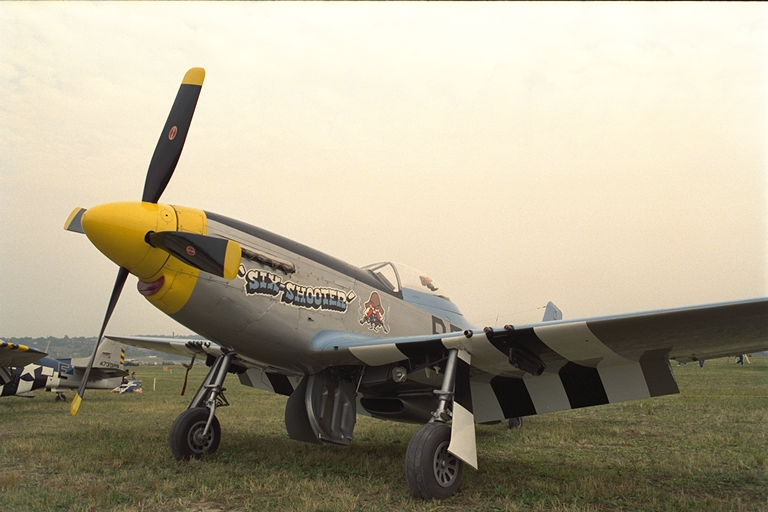
\includegraphics[width=0.5\textwidth]{imagenes/img9.png}
           \hfill
        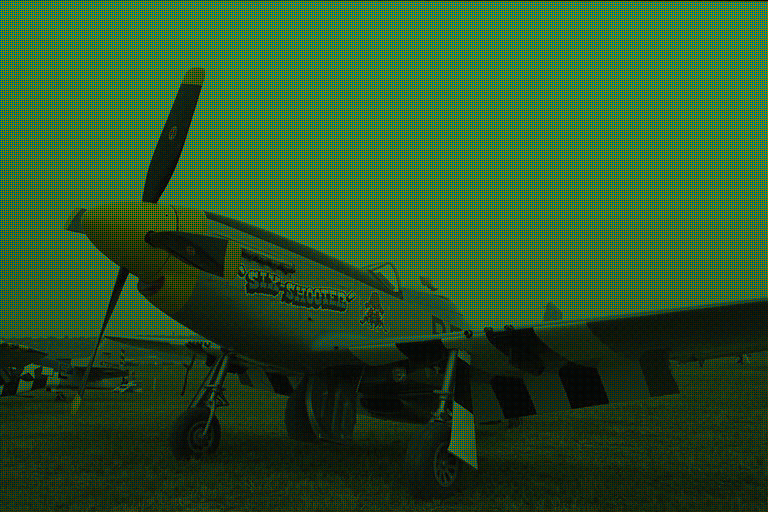
\includegraphics[width=0.5\textwidth]{imagenes/img9_bayer.png}
\end{figure}

\begin{figure}
       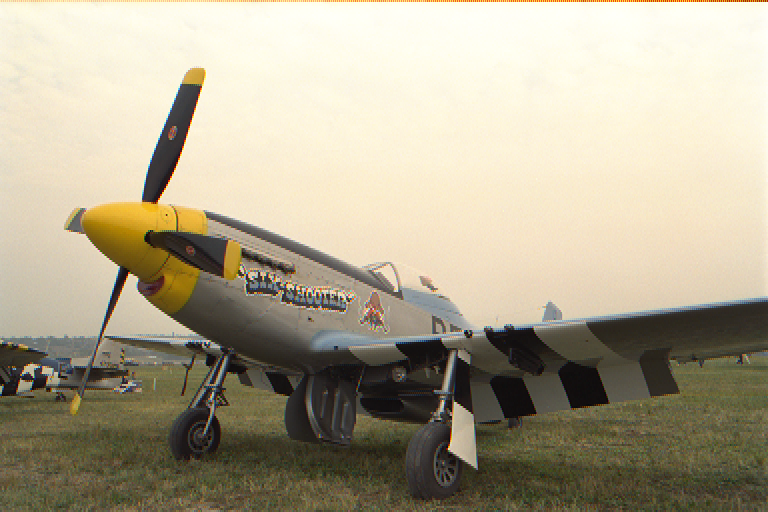
\includegraphics[width=0.5\textwidth]{imagenes/img9_demosicing_vecino.png}
           \hfill
        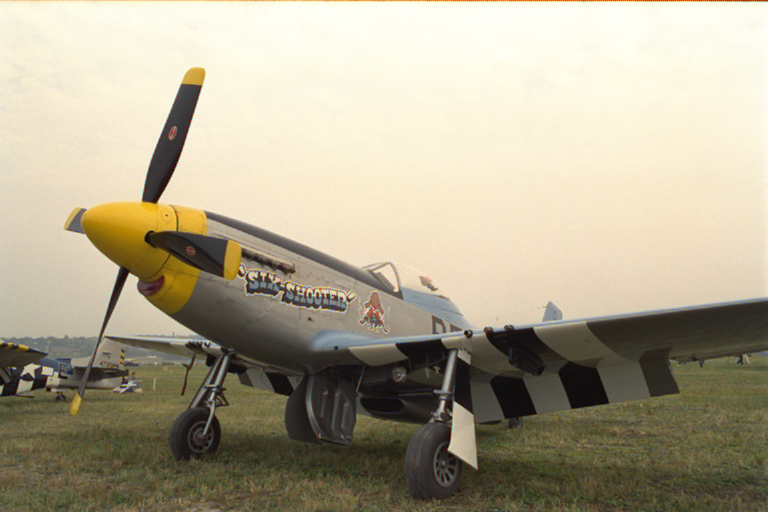
\includegraphics[width=0.5\textwidth]{imagenes/img9_demosicing_bilineal.png}
\end{figure}

\begin{figure}

       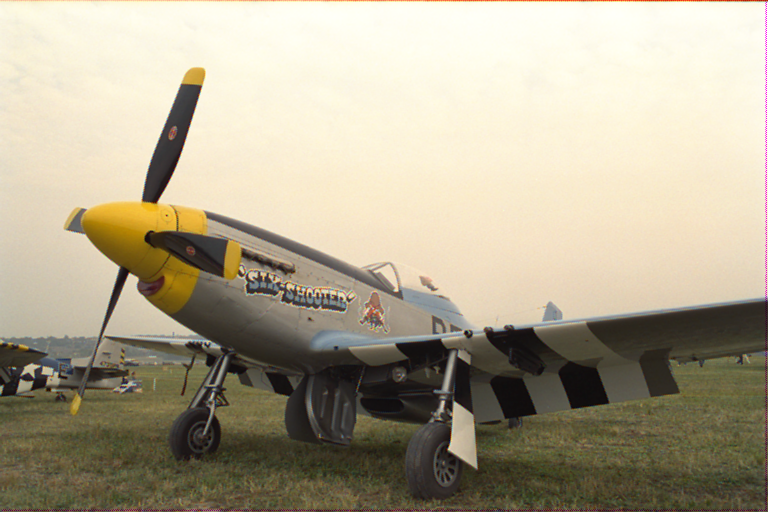
\includegraphics[width=0.5\textwidth]{imagenes/img9_demosicing_spline.png}
           \hfill
        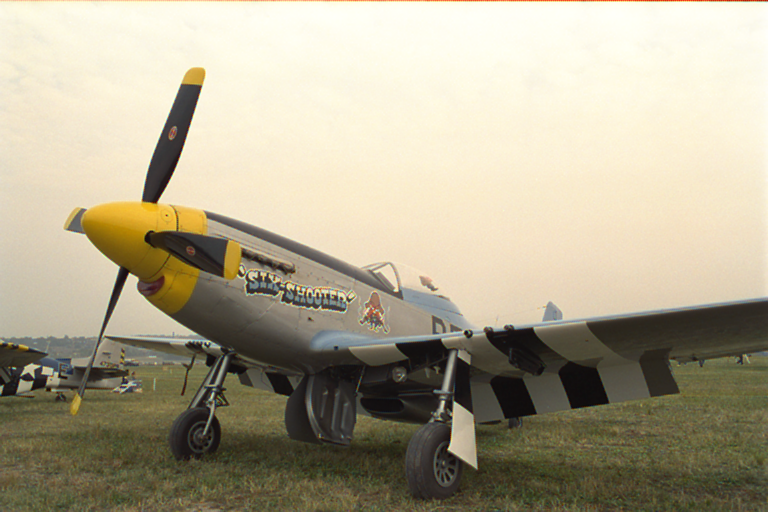
\includegraphics[width=0.5\textwidth]{imagenes/img9_demosicing_quality.png}
\end{figure}

\newpage

\subsection{Comparación de tiempos}

En esta sección presentaremos una comparativa entre los tiempos que tarda cada algoritmo a medida que aumenta el tamaño de la imagen. Para tal fin testamos cada algoritmo con imágenes cuadradas generadas aleatoriamente que van aumentando su tamaño, y creemos que es una forma correcta de comparar los tiempos ya que la complejidad de cada algoritmo es independiente de la información que tenga la imagen, pero dependiente del tamaño.

\begin{figure}[h]
       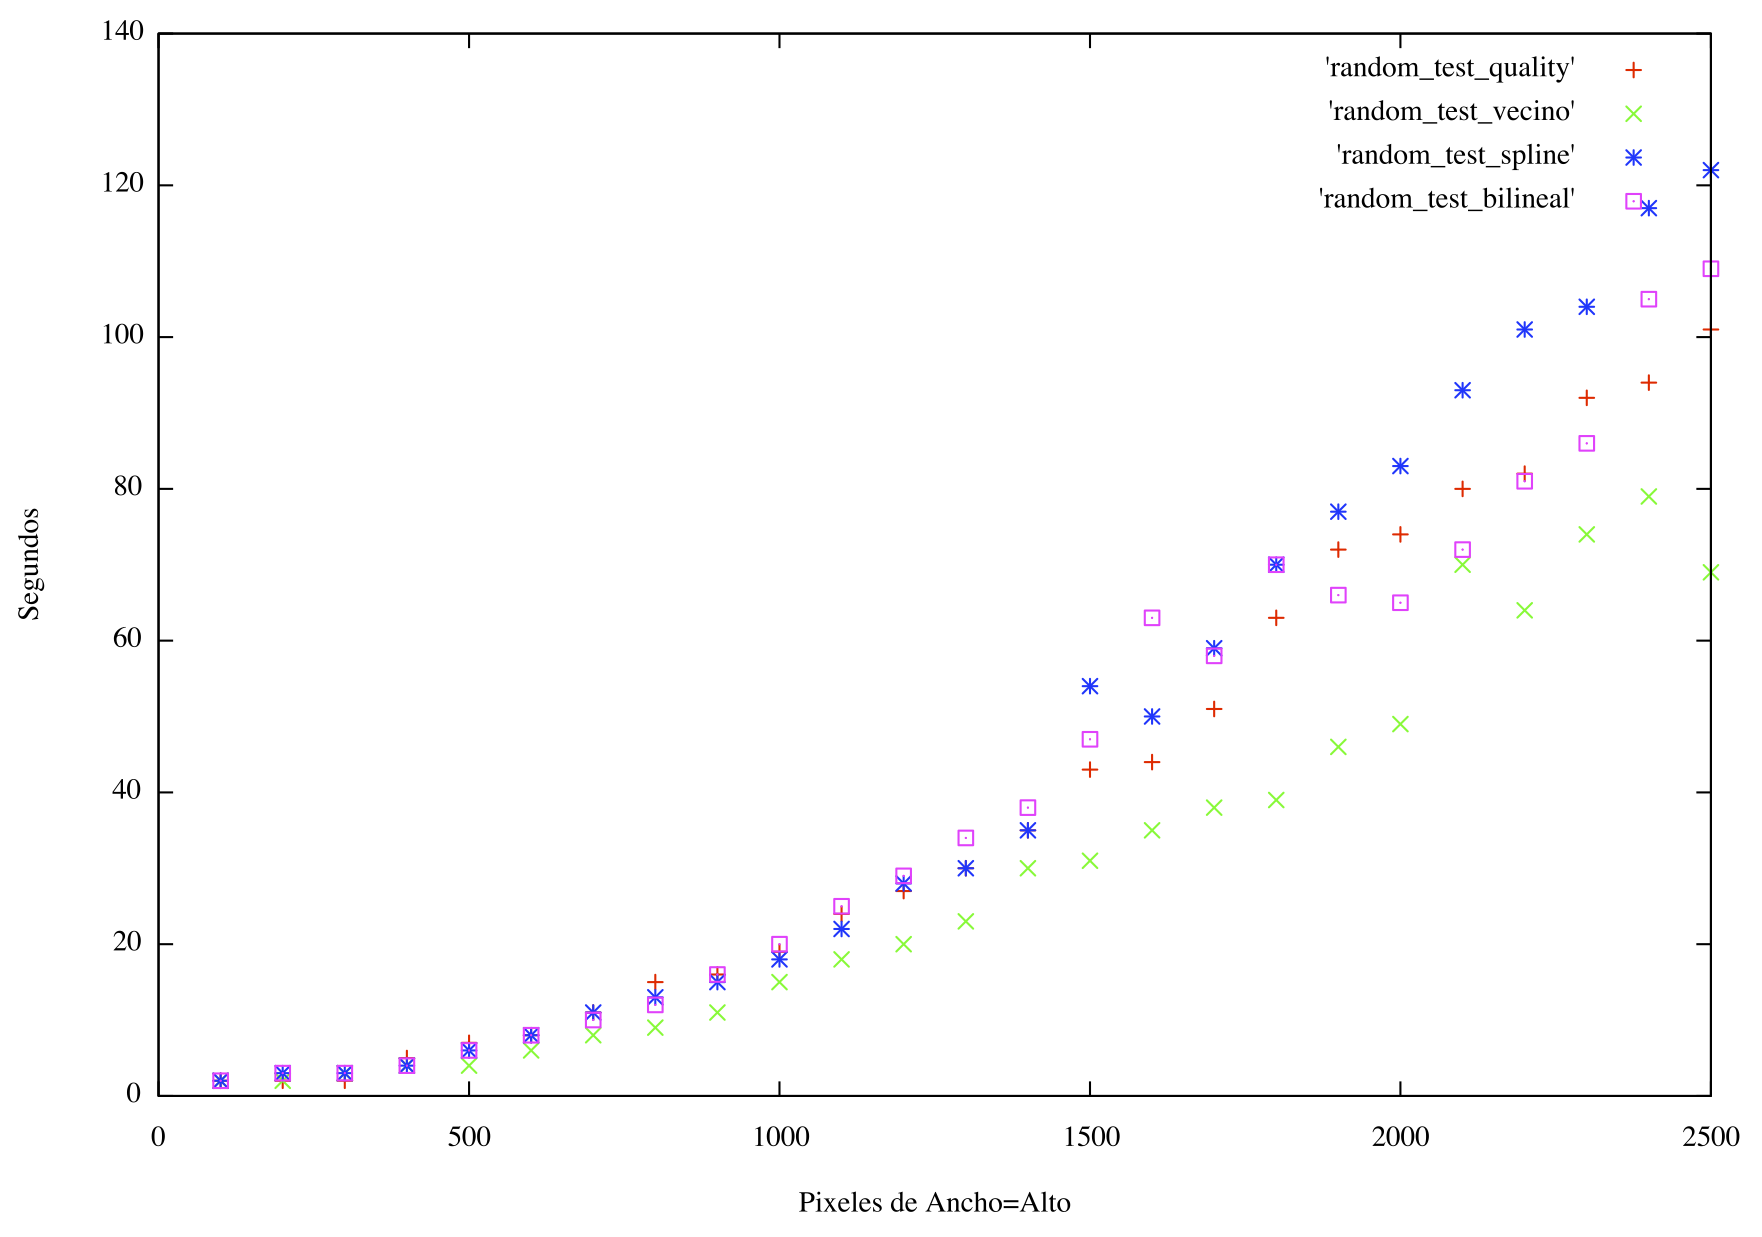
\includegraphics[width=1\textwidth]{imagenes/tiempo_algoritmos_random.png}
\end{figure}

\newpage

\subsection{Imagen 12}

A continuación probaremos con una imagen provista por la cátedra para tener mas resultados sobre los cuales apoyarnos a la hora de sacar nuestras conclusiones. Obviaremos la imagen bayerizada ya que sólo
nos interesaba ver que sea correcta la bayerización y con lo ya hecho eso queda claro.
\newpage
\begin{figure}
\begin{center}
       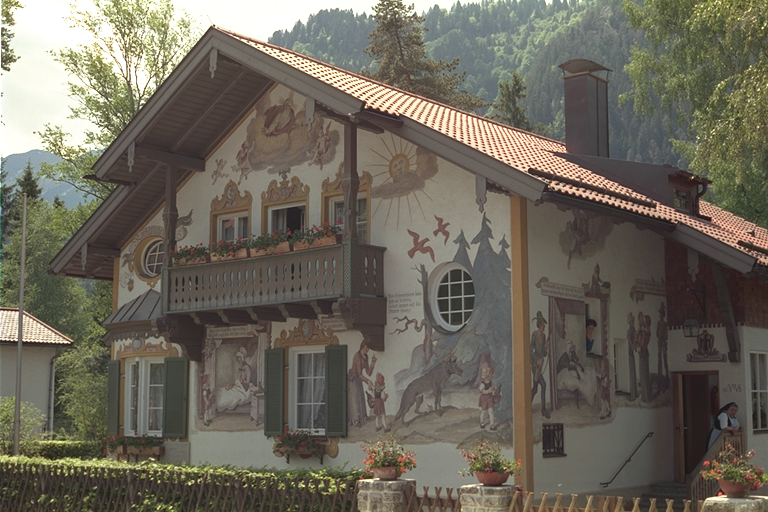
\includegraphics[scale=0.3]{imagenes/img12.png}
       \caption{Original }\label{fig:awesome_image1}
        \end{center}

\end{figure}

\begin{figure}[!htb]
\minipage{0.5\textwidth}
\begin{center}
    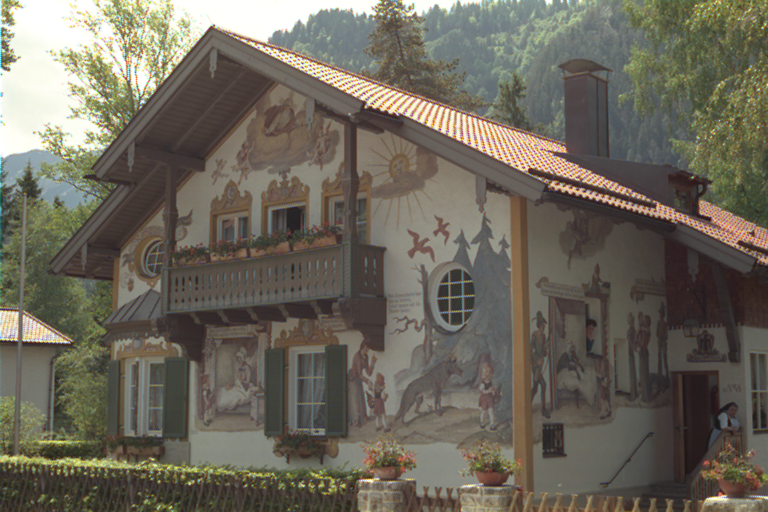
\includegraphics[scale=0.3]{imagenes/img12_demosicing_bilineal.png}
    \caption{Bilineal }
 \end{center}
\endminipage
\minipage{0.5\textwidth}
\begin{center}
    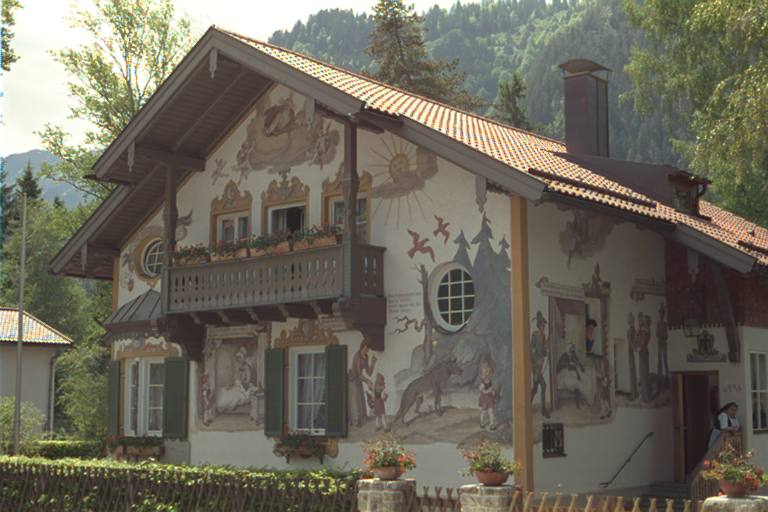
\includegraphics[scale=0.3]{imagenes/img12_demosicing_quality.png}
    \caption{High Quality}
        \end{center}
\endminipage\hfill
\end{figure}

\begin{figure}
\minipage{0.5\textwidth}
\begin{center}
    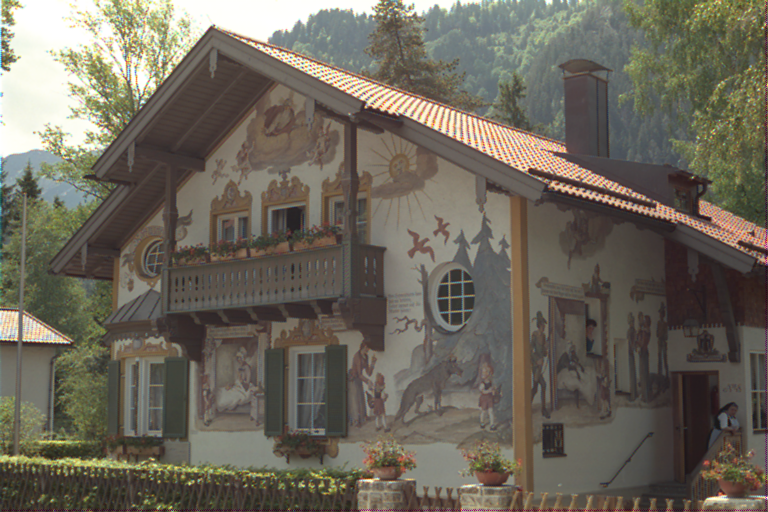
\includegraphics[scale=0.3]{imagenes/img12_demosicing_spline.png}
    \caption{Directional}
        \end{center}
\endminipage
\minipage{0.5\textwidth}
\begin{center}
    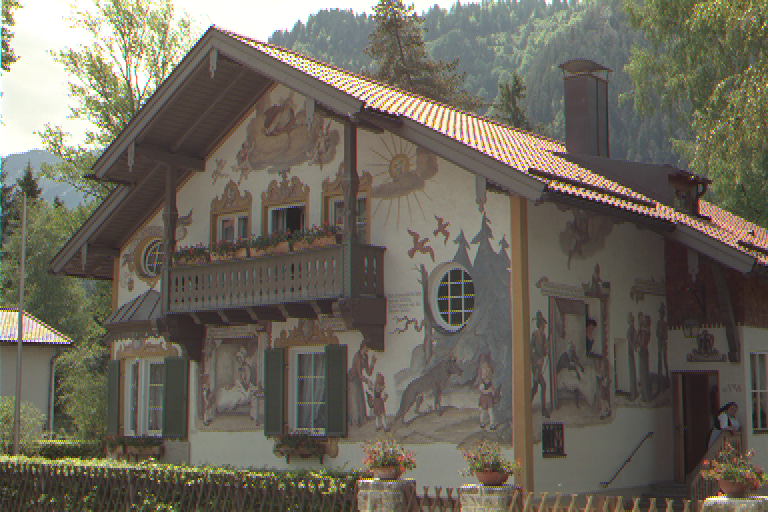
\includegraphics[scale=0.3]{imagenes/img12_demosicing_vecino.png}
    \caption{Vecinos}
 \end{center}
\endminipage
 
\end{figure}
\newpage

Subjetivamente highquality parece ser la mejor. Ya que se la ve bastante menos borrosa que las demás y con bordes mas nítidos, esto es facilmente apreciable en los dibujos que hay sobre la casa. A diferencia de vecinos que tiene bordes no sólo poco nítidos sino hasta claramente pixelados.

Veamos ahora a través del calculo del PSNR contra la imagen original cual es la mas mejor objetivoamente.


En el tejado de la casa podemos ver anomalías en todos los resultados, así como también en los arboles que estan a la izquierda y por encima. Más adelante analizaremos bien porque es que sucede esto.


\subsection{Comparación de calidad}
En esta sección compararemos solo los verdes de las imágenes y veremos los resultados utilizando PSNR. Recordemos que este término, calcula nivel de ruido en una señal.

\begin{figure}[h]
       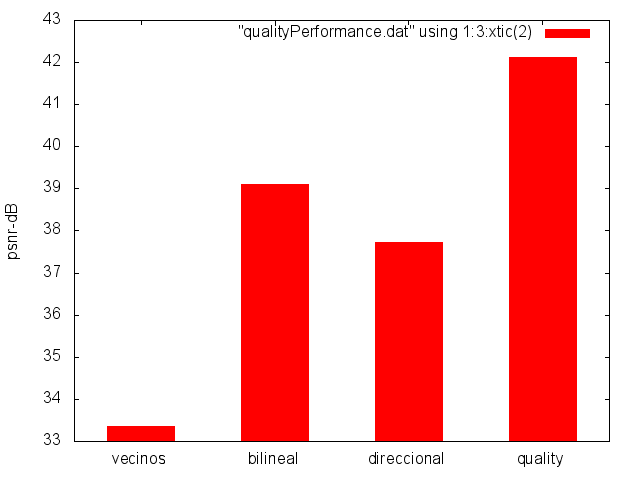
\includegraphics[width=1\textwidth]{imagenes/quality_performance.png}
\end{figure}

Como era esperado, el vecinos es el que peor hizo, y quality fue el mejor. Sin embargo notemos que Spline si bien tendría que tener un valor mayor que bilineal no lo tiene, es decir, el nivel de ruido es mayor en el direccional. Esto tiene sentido en la medida que el algoritmo direccional utiliza toda la fila y toda la columna para calcular el valor de las coordenadas $b_j$, $c_j$ y $d_j$ por lo que está sujeto a valores distintos al valor final, a diferencia de Bilineal que está sujeto a sus vecinos directos que es mucho más probable que tengan un valor más próximo.
  
